\documentclass{article}

% if you need to pass options to natbib, use, e.g.:
% \PassOptionsToPackage{numbers, compress}{natbib}
% before loading nips_2018

% ready for submission
\usepackage[preprint]{nips_2018}

% to compile a preprint version, e.g., for submission to arXiv, add
% add the [preprint] option:
% \usepackage[preprint]{nips_2018}

% to compile a camera-ready version, add the [final] option, e.g.:
% \usepackage[final]{nips_2018}

% to avoid loading the natbib package, add option nonatbib:
% \usepackage[nonatbib]{nips_2018}

\usepackage[utf8]{inputenc} % allow utf-8 input
\usepackage[T1]{fontenc}    % use 8-bit T1 fonts
\usepackage{hyperref}       % hyperlinks
\usepackage{url}            % simple URL typesetting
\usepackage{booktabs}       % professional-quality tables
\usepackage{amsfonts}       % blackboard math symbols
\usepackage{nicefrac}       % compact symbols for 1/2, etc.
\usepackage{microtype}      % microtypography
\usepackage{hyperref}
\usepackage{graphicx}

\title{Proposal for ECE285 project}

% The \author macro works with any number of authors. There are two
% commands used to separate the names and addresses of multiple
% authors: \And and \AND.
%
% Using \And between authors leaves it to LaTeX to determine where to
% break the lines. Using \AND forces a line break at that point. So,
% if LaTeX puts 3 of 4 authors names on the first line, and the last
% on the second line, try using \AND instead of \And before the third
% author name.

\author{
  Hongyuan Du \\
  PID: A53285631\\
  Department of Electrical and Computer Engineering\\
  UC San Diego\\
  \texttt{hdu@eng.ucsd.edu} \\
  %% examples of more authors
  %% \And
  %% Coauthor \\
  %% Affiliation \\
  %% Address \\
  %% \texttt{email} \\
  %% \AND
  %% Coauthor \\
  %% Affiliation \\
  %% Address \\
  %% \texttt{email} \\
  %% \And
  %% Coauthor \\
  %% Affiliation \\
  %% Address \\
  %% \texttt{email} \\
  %% \And
  %% Coauthor \\
  %% Affiliation \\
  %% Address \\
  %% \texttt{email} \\
}

\begin{document}
% \nipsfinalcopy is no longer used

\maketitle

\begin{abstract}
We are going to explore a new way that associate Generative Adversarial Networks (GANs) with style transfer techniques. We expect GANs with enhanced capacity can generate not only target contents, but also specific styles. Our goal is to learn a mapping $G: z \to I$, where $z$ is the domain of samples from low-dimensional latent variables, and $I$ is the domain of target images. The distribution of images from $G(z)$ should be indistinguishable both from the distribution of target content $C$ and the distribution of specific style $S$.
\end{abstract}

\section{Background}

A lot of brilliant works have been done on GANs and style transfer techniques and have achieved many impressive results. One of the most amazing works is \href{https://arxiv.org/pdf/1703.10593.pdf}{CycleGAN} proposed by Zhu et al., in which the authors implement a new structure of GANs to solve image-to-image translation problems. Our idea is inspired by CycleGAN, but what we will do is to come back to the origin of GANs --- to generate target samples from low-dimensional latent variables. We expect our generate network $G$ can create new images, not translate an image to another. This technique can be very useful in future artistic creation tasks, that just by manipulating low-dimensional parameters we can create artworks with desired contents and styles.

\section{Method}

In our project, we are going to propose new strategies for training GANs to enhance their capacity in capturing the distributions of contents as well as styles. So far, we have a very simple idea that firstly train the GAN with content images, and then enhance it by training with a style loss network. This idea is inspired by \href{https://arxiv.org/pdf/1603.08155.pdf}{fast-neural-style} technique proposed by Johnson et al., in which the authors use a CNN to approximate the style transfer mapping. In our work, we replace the CNN by GAN to achieve our goal. This change leads to different training strategy which we would like to describe it in detail in our final paper. We have done experiments that can generate promising images in 64x64 resolution which attached in \hyperref[ap]{appendix}. We are still working on the structure of our network and training strategy, and expect to get better results that generate higher resolution images.

We also have a more advanced idea that we want to improve our work by the idea from \href{https://arxiv.org/pdf/1606.03657.pdf}{InfoGAN} proposed by Chen et al., which make our latent variable interpretable separately for contents and styles, but we are not sure if we can realize it. We will try our best if there is enough time.

\section{Dataset}

Right now we are using \href{http://lsun.cs.princeton.edu/2017/}{LSUN} dataset to do our experiments, but we won't reject other datasets if we have time to try.

\newpage
\section*{Appendix}
\label{ap}

The output of the GAN we pre-trained on LSUN church-outdoor class:

\begin{figure}[!h]
\centering
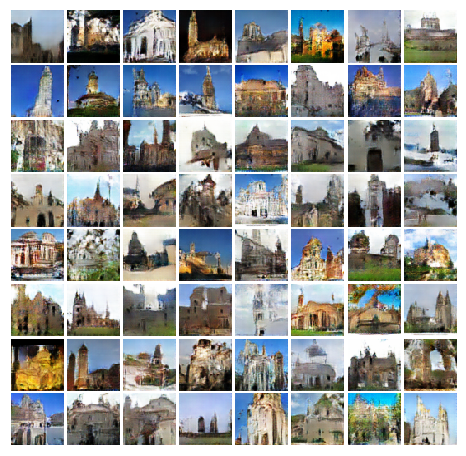
\includegraphics[width=0.7\textwidth]{../images/pretrained_gan_output.png}
\caption{Output of our pre-trained GAN on content images.}
\label{f1}
\end{figure}

Continue training the GAN with style loss network by $The\;Scream$ as the target style:

\begin{figure}[!h]
\centering
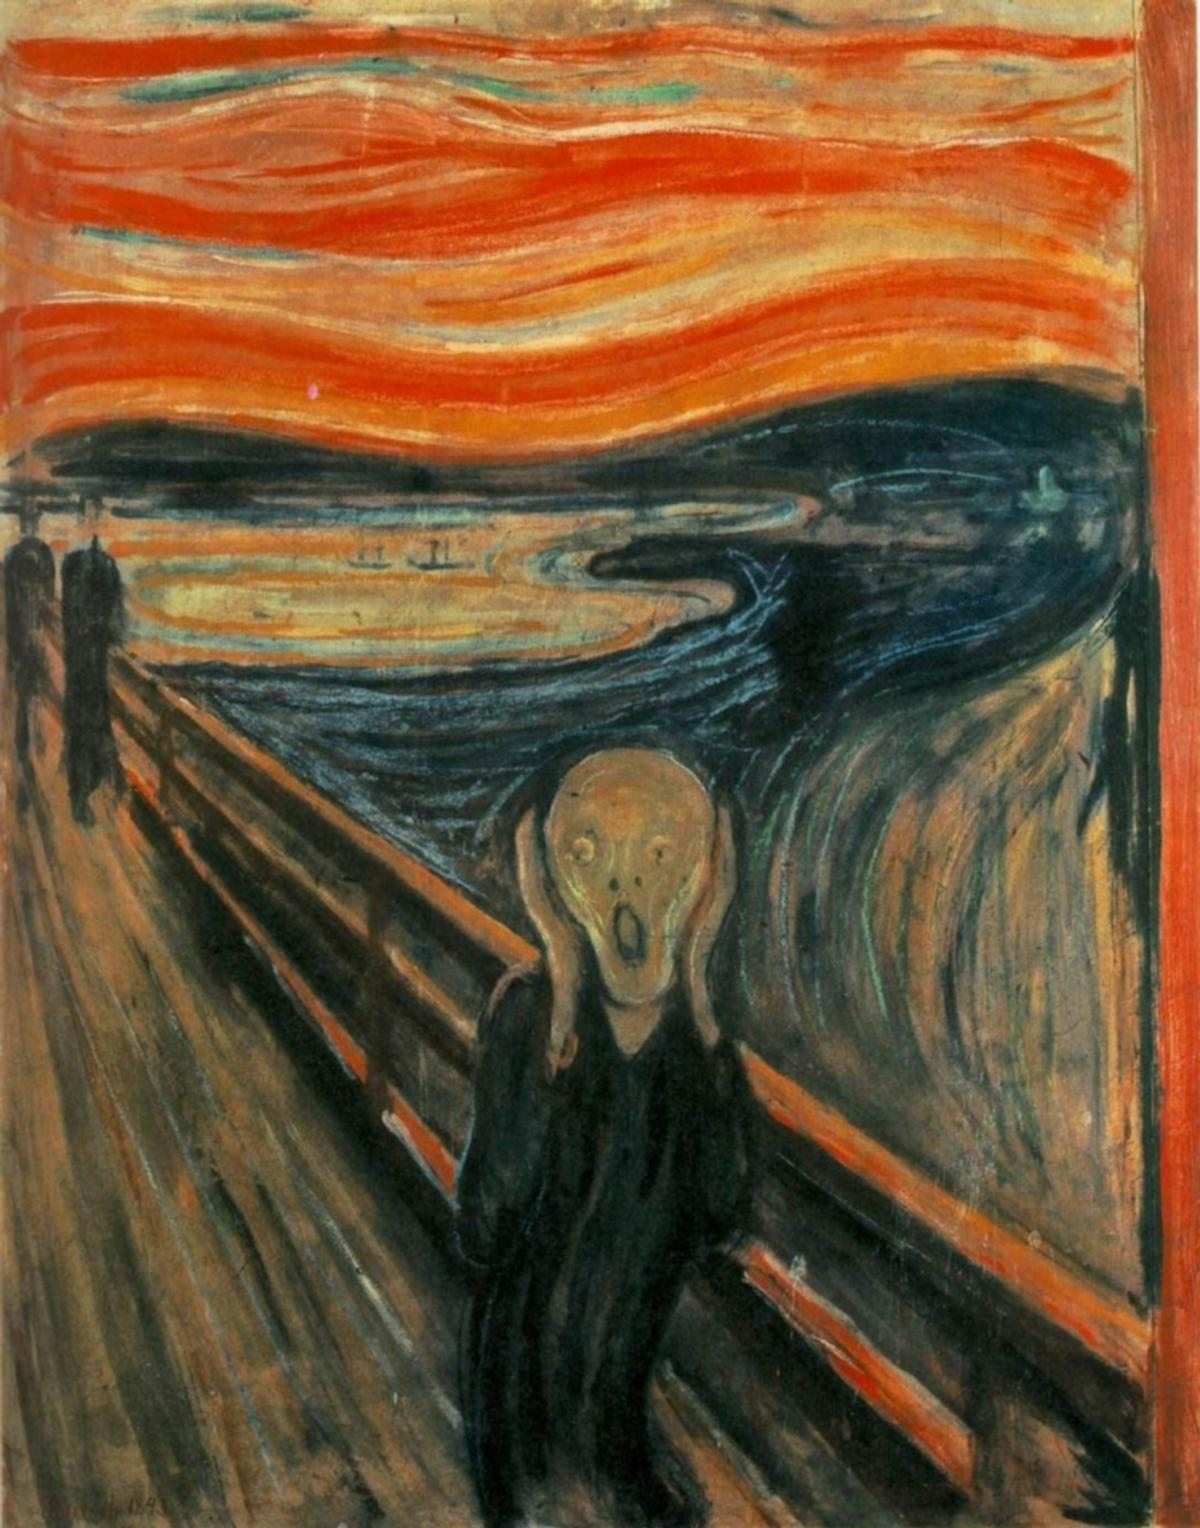
\includegraphics[width=0.4\textwidth]{../images/the_scream.jpg}
\caption{Target style.}
\label{f2}
\end{figure}

\newpage
Output of our StyleGAN:

\begin{figure}[!h]
\centering
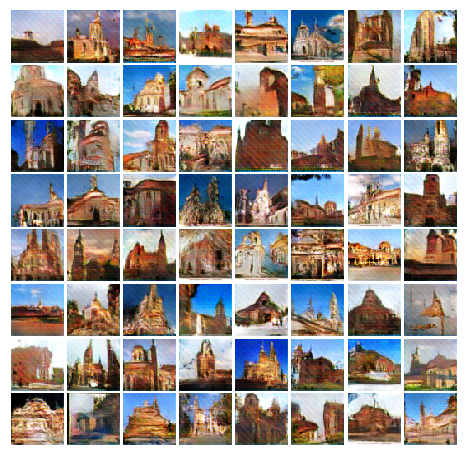
\includegraphics[width=0.7\textwidth]{../images/styleGAN_output.png}
\caption{Output of StyleGAN (lower learning rate).}
\label{f3}
\end{figure}

\begin{figure}[!h]
\centering
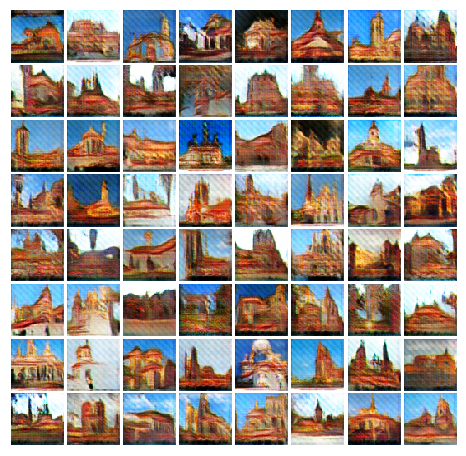
\includegraphics[width=0.7\textwidth]{../images/styleGAN_output2.png}
\caption{Output of StyleGAN (higher learning rate).}
\label{f4}
\end{figure}

\end{document}